% Chapter 1

\chapter{Introducción} % Main chapter title

\label{introduction} % For referencing the chapter elsewhere, use \ref{Chapter1} 

%----------------------------------------------------------------------------------------

% Define some commands to keep the formatting separated from the content 
\newcommand{\keyword}[1]{\textbf{#1}}
\newcommand{\tabhead}[1]{\textbf{#1}}
\newcommand{\code}[1]{\texttt{#1}}
\newcommand{\file}[1]{\texttt{\bfseries#1}}
\newcommand{\option}[1]{\texttt{\itshape#1}}
\newcommand{\lcdm}{$\Lambda$CDM }

%----------------------------------------------------------------------------------------


El origen de este trabajo iba a ser el estudio del modelo de crecimiento de galaxias bajo la influencia por una naturaleza \textit{warm dark matter} (WDM), en contraposición al modelo estandar asociado a la \textit{cold dark matter} (CDM). La finalidad era el estudio de la simulaciones de WDM pero debido al escaso cat\'alogo de estas simulaciones y el estatus de este trabajo se opt\'o por otro enfoque. Dicho enfoque pas\'o desde una perspectiva centrada a las simulaciones num\'ericas a un visi\'on m\'as te\'orica con la esperanza de poder ser traducida en un fut\'uro a una estado m\'as pr\'actico.\\

El objeto de este trabajo es el \textit{Impossible Early Galaxy Problem} (IEGP), definido por primera vez en el \textit{paper} \cite{steinhardt2016impossibly}, c\'omo la discordancia encontrada en ese mismo \textit{paper} sobre los datos deducidos de las observaciones de los campos CANDELS, SPLASH y CFHLS sobre la masa de los halos entre los redshift $4<z<7$ y los esperados por el modelo est\'andar (ver \textbf{Figura \ref{fig:stein16_f1}}). En dichas observaciones se encuentran un gran n\'umero de halos m\'uy masivos que quedar\'ian muy por encima de lo esperado por la función de masa de halo deducidad por el modelo cosmol\'ogico \lcdm y el modelo jer\'arquico de crecimiento gal\'actico. 

\begin{figure}[h]
	\begin{center}
	
		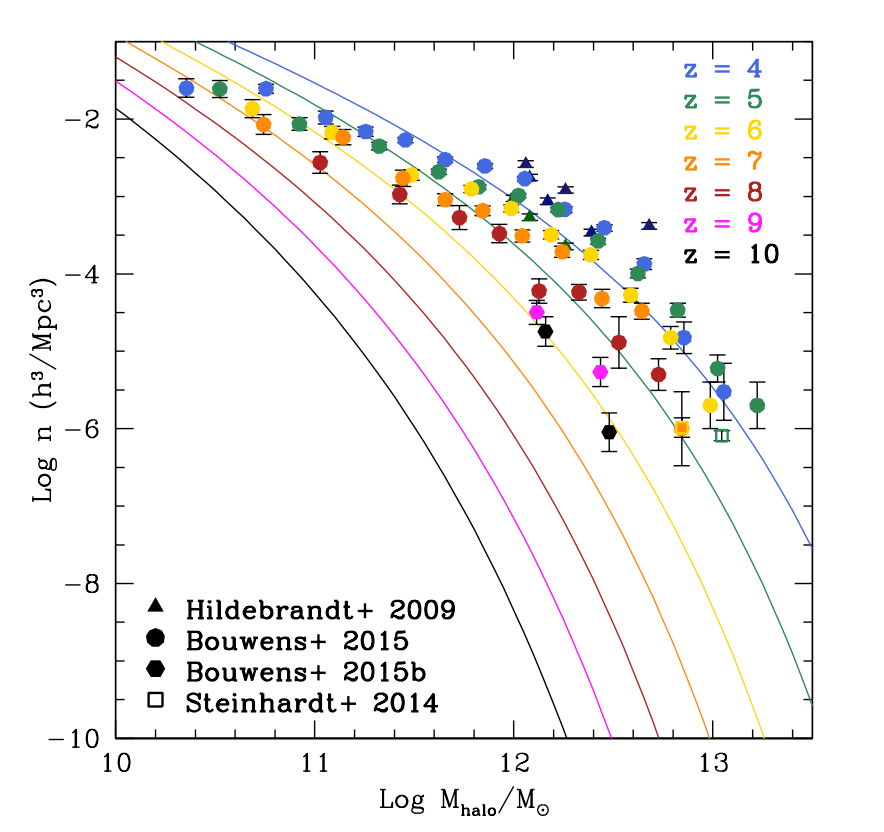
\includegraphics[scale=0.5]{Figures/steindhart_fig1}
		\caption{\label{fig:stein16_f1} Figura que representa la funci\'on de masa de halo. En l\'inea continua se muestra la predicci\'on te\'orica sacada de HMFCalc \citep{murray2013hmfcalc} y \cite{sheth2001ellipsoidal} mientr\'as que los marcadores muestran los valores obtenidos a trav\'es de las observaciones estudiadas en \cite{hildebrandt2009cars}, \cite{steinhardt2014uniform}, \cite{bouwens2015reionization} y \cite{bouwens2015uv}.}
		
	\end{center}
\end{figure}


El objetivo final de este trabajo pretende estudiar el problema IEGP desde tres enfoques distintos con la finalidad de clarificar cual puede ser el origen más plausible de las discrepancias observadas entre teoria y observaciones que parecen mostrar la \textbf{Figua \ref{fig:stein16_f1}}. Estos enfoque son:
\begin{description}
	\item[Observacional:] ¿Qué \textit{bias} observacionales pueden estar presentes? ¿Existen otros posibles \textit{bias} observacionales que no se hayan podido tomar en cuenta? ¿Hay otro tipos de sesgos que se hayan podido cometer al calcular la función de masa de halo de las observaciones consideradas? Desde esta perspectiva se pretenderá analizar el problema y determinar si tiene un papel relevante en la discrepancias observadas. También si nuevas observaciones y simulaciones contribuyen de manera positiva o negativa en este punto como por ejemplo los trabajos \cite{wang2019dominant} o \cite{behroozi2019universemachine}.
	
	\item[Física Bariónica:] Son muchos los trabajos que consideran que los procesos físicos de la matería bariónica podrían variar en función del redshift haciendo más eficiente, por ejemplo, los procesos de \textit{feedback} de AGNs que propicián la inhibición del SFR en redhift bajos \citep{finkelstein2015increasing}. Las recetas de la física bariónica juegan un papel fundamental en la relación entre masa estelar \textit{v.s} la masa del halo (SMHMR), veremos si son relevantes en este problema como parece plantear el trabajo de \cite{finkelstein2015increasing} o si por el contrario son suprimibles en el IEGP simplificando un poco el problema.
	
	\item[Modelo Cosmológico:] Por regla general y según ha marcado la experiencia de la historia científica, cuando existe una discrepancia entre observación y teoría suele ser el segundo factor el que está equivocado. Son muchos los logros del \lcdm pero también existen muchos problemas no explicados por este modelo y el IEGP parece convertirse en otro más. Daremos un repaso de los problemas que parece no explicar el \lcdm e intentaremos estudiar el IEGP considerando otros modelos cosmógicos y naturaleza de materia oscura que se encuentran sobre la mesa de teorías aceptadas o con el estatus de encontrase en consideración debido a las posibles carencias del \lcdm.
\end{description}


En esta primera sección daremos un pequeño resumen de los principales puntos del \textit{paper} de \cite{steinhardt2016impossibly} comparando de manera conjunta los resultados con los que se derivarían de las nuevas medidas ofrecidas por \cite{behroozi2019universemachine}, en un intento de ver si datos más actualizados pueden contribuir a solucionar o agravar las discrepancias observadas. En las siguientes secciones abordaremos de manera independiente los tres enfoques explicados terminando con una última sección dedicada a las conclusiones y a los posibles fututos trabajos que se podrían realizar en el campo de las simulaciones en aras de clarificar este problema . Pero lo primero es explicar el problema y allá vamos.


\section{\textit{The Impossible Early Galaxy Problem}.}

Existe un consenso bastante amplio en el que en un escenario basado en el modelo cosmológico \lcdm las grandes masas finales de los halos predichos por la función masa de halo cambian rápidamente entre los redshift 8 y 4, cuyos halos que contienen a las galaxias más masivas virializan hacia z=4 \citep{steinhardt2016impossibly}. Sin embargo, no se han encontrado evidencias de esa evolución esperada entre los rangos de redshift mencionados, por ejemplo, trabajos como el \cite{finkelstein2015increasing} y \cite{finkelstein2015evolution} han deducido una independencia del valor de la magnitud UV característica $M^*_{UV}$ de la función de  parametrización de Scheter con respecto al redshift en los rangos z$\in [4,7]$, por tanto, sin encontrar signos de una evolución esperada entre las galaxias de estos redshift. Dichos trabajos encontraron un mayor número de galaxias brillantes en UV de lo esperado en redshift z=7, que concuerda con el resultado de \cite{steinhardt2016impossibly} y que se puede visualizar en la \textbf{Figura \ref{fig:stein16_f1}}. En \cite{steinhardt2016impossibly} compara las funciones de masa de halo obtenidas de los trabajos de \cite{hildebrandt2009cars}, \cite{steinhardt2014uniform}, \cite{bouwens2015reionization} y \cite{bouwens2015uv} calculadas basándose en las observaciones de los estudios de CANDELS\footnote{\cite{grogin2011candels}}, CFHTLS\footnote{\cite{hildebrandt2009cars}} y SPLASH\footnote{\cite{capak2012splash}} y usando tres metodologías distintas que explicaremos en la siguientes subsecciones, con las funciones de masa de halo predichas por modelos teóricos obtenidos de la herramienta \textit{HMFCalc} \citep{murray2013hmfcalc} usando como base el trabajo de \cite{sheth2001ellipsoidal} y que explicaremos con un mayor detalle más adelante. Las discrepancias que se pueden observar en la \textbf{Figura \ref{fig:stein16_f1}} son muy notables y estudiadas en \cite{steinhardt2016impossibly}, aquí haremos un pequeño resumen de estas explicaciones aplicando nuevas medidas y observaciones obtenidas principalmente de \cite{behroozi2019universemachine} y \cite{wang2019dominant}, sin embargo, existen posturas contrarias a la existencia de tal problema. Trabajos como el de \cite{behroozi2018mostmassive} afirman que tal problema no existe ya que los ratios de masa estelar - masa bariónica considerados en \cite{steinhardt2016impossibly} del $9\%$ pueden ser superiores para los rangos de redshift entre $z=4-8$, llegando a encontrarse entre el 10\% y el 40\% con un error de $0.2\mathrm{dex}$ por lo que no sería descartable la aparición de ratios cercanos a la unidad (Ver \textbf{Figura \ref{fig:beh-silk-2010-fig1}}). Por el otro lado, las observaciones presentadas en \cite{wang2019dominant} de galaxias masivas invisibles al óptico e infrarrojo cercano parece que debiera aumentar el numero de densidad de estas galaxias aumentando la masa de estos cúmulos de por si ya masivos, aunque esto podría ser solo un indicativo del aumento de la masa estelar y por tanto un aumento del ratio SMHM favoreciendo la concordancia entre la teoría y las observaciones. \\

\begin{figure}[t]
\centering
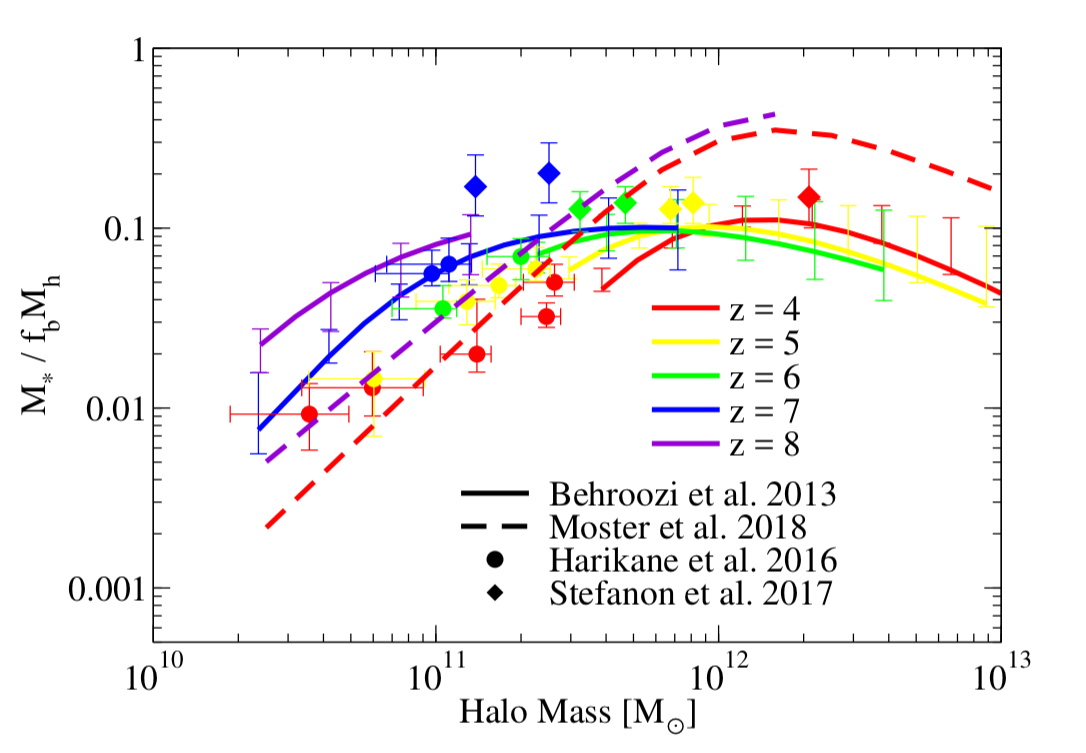
\includegraphics[scale=0.5]{Figures/Behroozi-silk_2010_fig1}
\caption{\label{fig:beh-silk-2010-fig1}. Ratios de masa estelar-masa bariónica para un rango de redshift $z= 4-8$ que alcanzan niveles entre el 10\% y el 40\%. Con una dispersión de $0.2\mathrm{dex}$ es plausible que galaxías individuales puedan alcanzar ratios cercanos a la unidad. Los resultados han sido reconvertidos a la IMF de Salpeter y a los parámetros cosmológicos de Planck 2016. Las medidas de Behroozi et al. (2013), Stefanon et al. (2017) y Moster et al. (2018) usan la técnica de enlace de abundancias; mientras que Harikane et al. (2016) usa modelos de la distribución anular de ocupación del halo. Imagen sacada de \cite{behroozi2018mostmassive}}
\end{figure}


\textcolor{blue}{El conflicto que aparece en el trabajo de \cite{steinhardt2016impossibly} es la presencia un gran número inesperado de halos de materia oscura en redshift altos. Esto esta medido a través del número de densidad de galaxias masivas debido al hecho que podemos ver en Mo que las galaxias masivas están presentes en los halos masivos y viceversa. Para detectar la masa de las galaxias que se hospedan en los halos de materia oscura podemos recurrir a dos procedimientos: uno es el de clusterización que se basa principalmente en la medida de la función de correlación de galaxias representado en el trabajo de \cite{hildebrandt2009cars} y el otro es la medida de la masa estelar. Dado que la masa estelar es complicada a medir en estos redshift se usa la relación que existe con la función de luminosidad en UV, lo cual es un indicativo de la SFR. Esto último implica varios problemas, el primero es el representado por los resultados de \cite{wang2019dominant} donde presenta medias de galaxias textit{invisibles} al infrarrojo cercano y óptico las cuales contienen gran cantidad de polvo y son muy representativas en estos redshift en las galaxias más masivas. Los otros problemas los tengo que revisar pero sería que el SFR varía con el redshif y que las galaxias mas masivas de $>10^{13}M_{\odot}$ presentan un amortiguamiento del SFR (masa mágica), lo cual nos las estaríamos dejando fuera. Quizás estas últimas galaxias no son representativas pero no entiendo muy bien porque las están dejando fuera, quizás por que esta relación de apagado del SFR no se presenta en estos redshift}.\\

\textcolor{blue}{Por otro lado existen maneras de medir la masa de un halo sin medir la masa de las galaxias como las obtenidas por lentes gravitacionales o movimiento cinemático de las galaxias de los cúmulos. Veamos como encajamos todo esto en el problema.}

\textcolor{green}{Los siguientes pasos a seguir son el estudio de los argumentos de \cite{behroozi2018mostmassive} y ver como encajamos las medidas de \cite{wang2019dominant} con las de \cite{behroozi2019universemachine} en el problema}

\textcolor{red}{Las medidas presentadas por \cite{steinhardt2016impossibly} las podemos dividir en dos grupos. La primeras, las medidas de \cite{bouwens2015uv} usando las técnicas de enlace de abundancias parecen tener dos posibles problemáticas basada en el ratio de masa estelar-masa bariónica considerado del 9\%, el cual según trabajos de Behroozi pueden ser superiores (\cite{behroozi2018mostmassive},\cite{behroozi2019universemachine}) y el otro es el de la masa estelar no observada presentado por \cite{wang2019dominant}. Estos dos problemas podrían combinarse para aumentar el SMHM lo que devolvería  las observaciones al campo de la teoría.} \\

\textcolor{red}{Por otro lado, las observaciones de \cite{hildebrandt2009cars} también salen bastante desviadas de la teoría, tendríamos que ver cuales pueden ser las posibles razones. Los siguientes pasos a seguir sería desarrollar el punto anterior y ver las causas de este. Por último ver las diferentes casuísticas tomando distitas cosmologías sobre todo la Fuzzy Dark Matter y la teoría MOND.}\\

Estos problemas los afrontaremos con las últimas medidas presentadas en \cite{behroozi2019universemachine} para tener los datos más actualizados posibles por lo que es de interés hacer un pequeño repaso a lo presentado en este trabajo y resaltar los resultados de interés para nuestro dilema que podemos encontrar en él.

\subsection{\textit{Universe Machine}}

En el trabajo de \cite{behroozi2019universemachine} se presenta una serie de resultados derivados de la obtención de las estimaciones de la función de masa estelar, ratio de formación estelar cósmica y específica, la función de luminosidad UV, las fracciónes de amortiguamiento, funciones de autocorrelación, relación de masa estelar \textit{v.s.} UV y la relación IRX-UV determinadas a traves de simulaciones \textit{Marckov Chain Monte Carlo} (MCMC) usando los datos observacionales de los estudios de CANDELS, 3D-HST, ULTRAVISTA y ZFOURGE y las simulaciones de materia oscura de \textit{Bolshoi-Planck} y \textit{MDPL2}. Sin entrar en detalle en la explicación de la metodología (nos remitiremos a \cite{behroozi2019universemachine}) daremos un pequeño esbozo de la metodología usada en estas simulaciones MCMC.\\

\begin{figure}
	\centering
	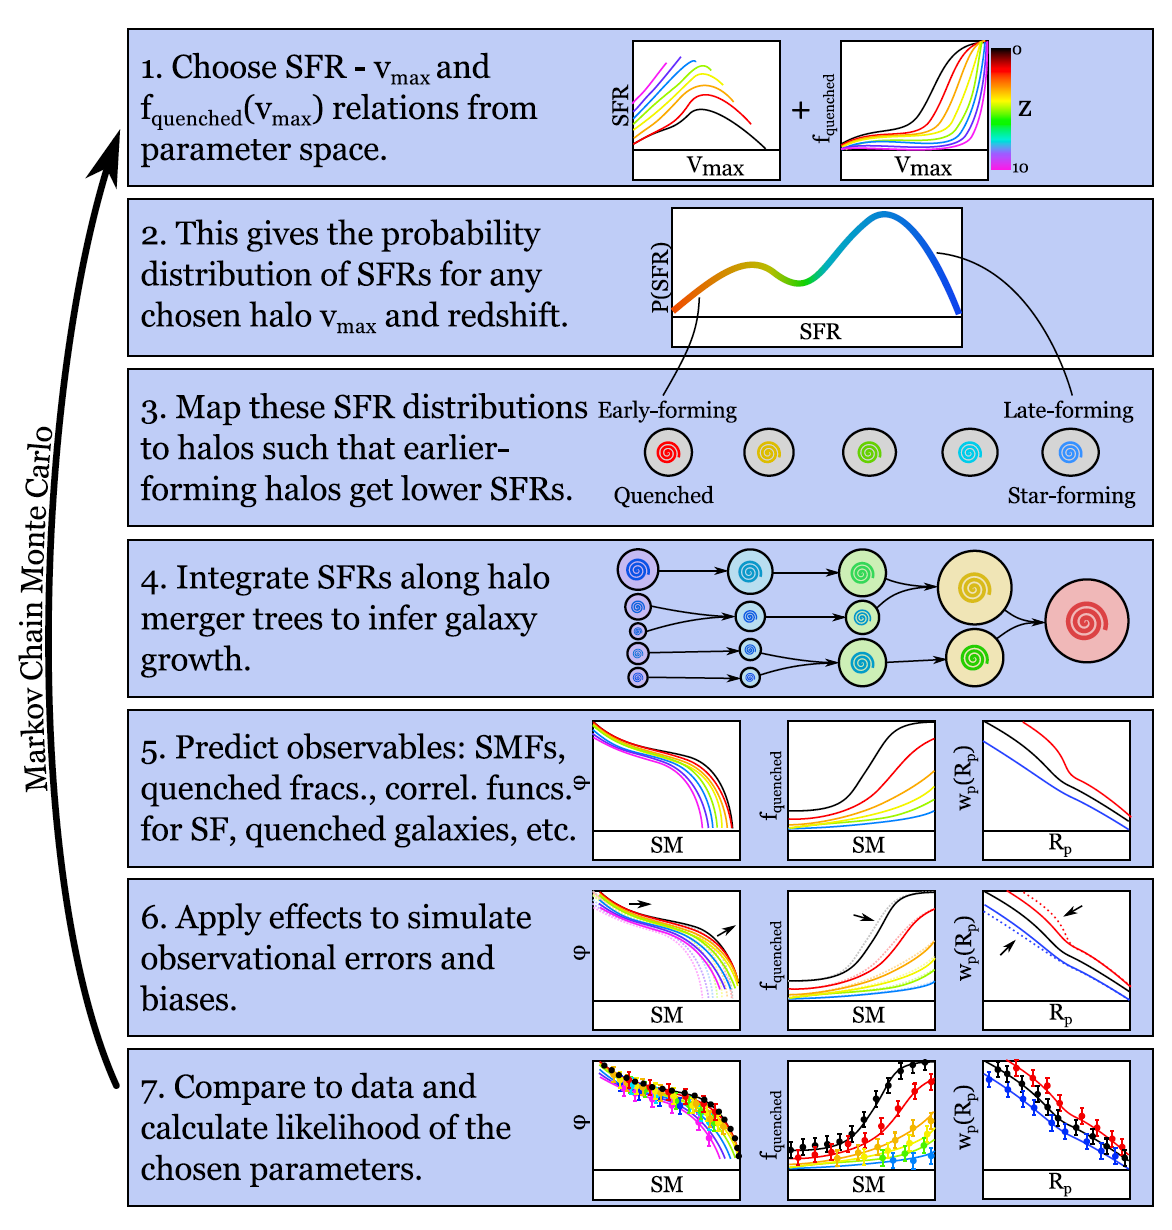
\includegraphics[scale=0.5]{Figures/behroozi_mcmc}
	\caption{\label{fig:behroozi_mcmc} Resumen del método usado en \cite{behroozi2019universemachine} para enlazar el crecimiento galáctico con el del halo.}
\end{figure}

El método a grades rasgos está recogido en la \textbf{Figura \ref{fig:behroozi_mcmc}} y en  el cual no se considera una correlación \textit{a priori} entre la acrección de la galaxia y la del halo. En este método se genera un universo \textit{mock}, basádo en los árboles de fusiones sacados de las simulaciones de materia oscura de \textit{Bolshoi-Planck} y se comparan a traves de funciones de verosimilitud bayesianas con las observaciones reales. A través de un algoritmo MCMC se vuelve a generar el universo \textit{mock} y se vuelve a realizar la misma comparación obteniendo nuevas funciones de verosimilitud bayesianas. \\

Los resultados más interesantes en lo que respecta a este trabajo los intentaremos explicar en profundidad a continuación para luego posteriormente compararlos con las mediciones presentadas en \cite{steinhardt2016impossibly}

\subsubsection{Relación masa estelar - UV} 
Las medidas dadas por \cite{bouwens2015reionization} y \cite{bouwens2015uv} representadas en la \textbf{Figura \ref{fig:stein16_f1}} están basadas en el trabajo de \cite{finkelstein2015increasing}, el cual se basa en la técnica del \textit{emparejamiento} de halo y galaxias para obtener la relación masa halo - luminosidad UV. Más adelante se explicará en que consiste exactamente esta técnica, pero lo interesante a saber en lo que respecta a este punto es que depende de manera intermedia en la relación masa estelar - luminosidad. Dicha relación es revisada en \cite{behroozi2019universemachine} dando nuevos valores que dejan por encima a las estimaciones de \cite{finkelstein2015increasing},\cite{finkelstein2015evolution} como se muestra en la \textbf{Figura \ref{fig:cstm_behroozi_uvsm}}.  \textcolor{red}{Esto podría ocasionar dos opciones antagónicas pero con el mismo origen de un descenso de la masa estelar. Si el SMHM se mantuviese fijo bajaría la masa del halo reconciliando la teoría con las observaciones mientras que si lo que ocasiona es una caida del SMHM podría ocasionar el efecto inverso, siendo mayor el problema de lo que es. Sin entrar en las observaciones de Wang. }
 
\section{Datos Observacionales}
Como ya se ha comentado, el trabajo de \cite{steinhardt2016impossibly} divide las estimaciones de la masa de halo de los diferentes campos observados en tres grupos según la técnica usada. Como se recalca en el \textit{paper} \cite{steinhardt2016impossibly} la ventaja de trabajar en redshifts altos es que nos permite ver diferentes fotogramas del universo con un intervalo más corto entre ellas que si la viésemos en rangos más bajos. En nuestro caso el rango medio del intervalo de tiempo entre los redshift 4 y 7 son de 0.9 giga-años, esto nos permite mediciones entre épocas más precisas aunque a cambio nos restringe bastante en los métodos disponibles para calcular la masa de halo de estos rangos, \cite{steinhardt2016impossibly} usa tres representados por diferentes \textit{papers}:
\begin{itemize}

	\item Un método es el presentado y desarrollado en el artículo de \cite{finkelstein2015increasing}, el cual se basa en la curva de luminosidad UV y en la función de masa calculada a través de simulaciones de Bolshoi, relacionando ambas por el principio de que el halo más masivo a de albergar la galaxia más masiva y viceversa. Las mediciones plasmadas en la \textbf{Figura \ref{fig:stein16_f1}} de los estudios de \cite{bouwens2015reionization} y \cite{bouwens2015uv} usan esta técnica.

\item En el trabajo de \cite{hildebrandt2009cars} se muestra el método de clusterización, el cual estima la masa del halo según la distribución espacial de las galaxias. La ventaja de este método es que no hay que asumir ninguna propiedad físicas de las galaxias, pero sí es necesario escoger un modelo de materia oscura para las simulaciones.

	\item El último método es asumir un ratio entre luminosidad/masa estelar y materia oscura. El ratio asumido es el redshift más bajos donde las estimaciones de materia oscura son más factibles por los métodos de agrupación. El ratio usado para el enlace entre masa estelar y de halo es $M_h/M_\star \sim 70 $ siendo la técnica usada en las mediciones de \cite{steinhardt2014uniform} que se presentan en la \textbf{Figura \ref{fig:stein16_f1}}.
\end{itemize}

Discutiremos estas tres técnicas por separado actualizando las medidas con los nuevos datos de \cite{behroozi2019universemachine}, pero antes de ello hagamos una pequeña presentación del trabajo de \cite{behroozi2019universemachine}.


	

\begin{figure}[h]
	\begin{subfigure}{.5\textwidth}
  		\centering
  		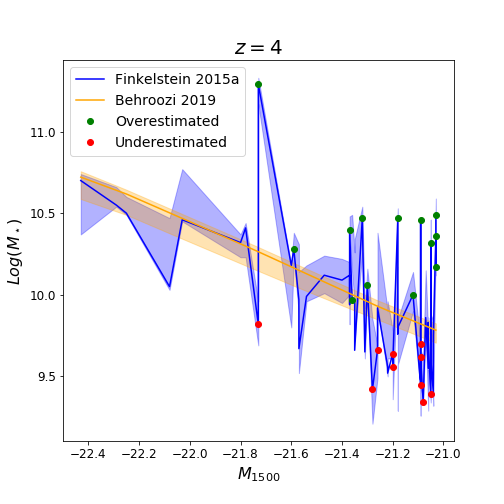
\includegraphics[width=1.1\linewidth]{Figures/sm-uv/z_4.png}
  		\label{fig:sfig1}
	\end{subfigure}%
	\begin{subfigure}{.5\textwidth}
  		\centering
  		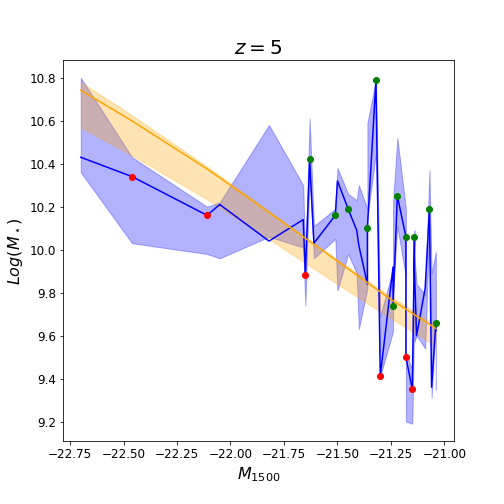
\includegraphics[width=1.1\linewidth]{Figures/sm-uv/z_5.png}
  		\label{fig:sfig2}
	\end{subfigure}
	\begin{subfigure}{.5\textwidth}
  		\centering
  		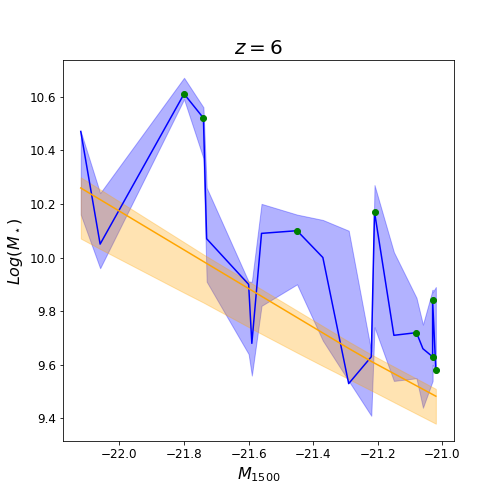
\includegraphics[width=1.1\linewidth]{Figures/sm-uv/z_6.png}
  		\label{fig:sfig3}
	\end{subfigure}%
	\begin{subfigure}{.5\textwidth}
  		\centering
  		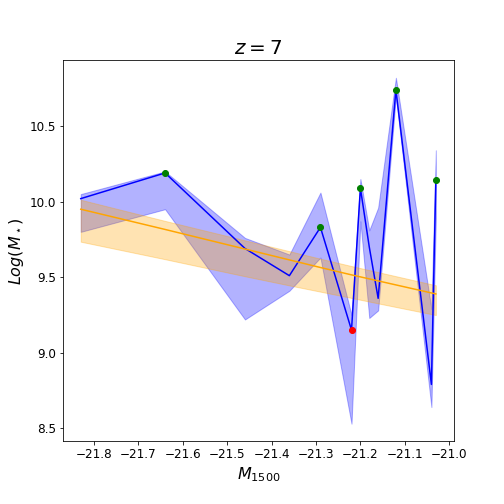
\includegraphics[width=1.1\linewidth]{Figures/sm-uv/z_7.png}
  		\label{fig:sfig4}
	\end{subfigure}
	\caption{\label{fig:cstm_behroozi_uvsm} En la figura se representa la función que relaciona la luminosidad UV y la masa estelar del trabajo de \cite{finkelstein2015increasing} \textit{v.s.} el resultado obtenido por el trabajo de \cite{behroozi2019universemachine}. Las observaciones son las usadas por \cite{finkelstein2015increasing} en el que representamos los intervalos de confianza de cada uno de los estudios. Hemos pintado en rojo aquellas mediciones de \cite{finkelstein2015increasing} que quedán por debajo del intervalo de confianza de las mediciones de \cite{behroozi2019universemachine} y en verde aquellas que quedan por encima.}
\end{figure}



\subsubsection{Relación masa halo - masa estelar} Uno de los resultados más interesantes según el propósito de este trabajo es el estudio de la relación masa halo - masa estelar para el rango de redshift del estudio $z\in [0,10]$. Se encuentra que el ration SMHM varía entre galaxias satélite y galaxias centrales, por ejemplo en halos menos masivos le ratio de SMHM es mayor en las galaxias satélite ya que su tiempo de ``apagado''  es más largo creciendo en masa estelar mientras que permanece fija en su masa de materia oscura. Por otro lado en masas de halo altas el canal principal de crecimiento es via fusiones donde en las galaxias satélite es menos frecuente dando ratios de SMHM más bajos que en las galaxias centrales. La imagen del SMHM se complica en masas intermedias 

\subsection{Método de función de luminosidad UV}
	
\subsection{Método de Clusterización}

\subsection{Método de ratio luminosidad masa halo}

\section{Normalidad de las Galaxias}

